\begin{frame}
	\frametitle{SHA-256}
	\framesubtitle{Secure Hash Algoritm 256 bit}
	
	\begin{itemize}	 
			\item $\sfrac{256}{2}=$ {\color{blue}128 bit di sicurezza}\;\;\; collisioni non ancora trovate 
			\item $\mathrm{len}(m)< 2^{64},\;\;\;\;\;\;\;\;\;\;\; \text{len}(n)=256$
	\end{itemize}

	\begin{columns}
	 \begin{column}{.65\textwidth}
		\begin{enumerate}	 
		  	\item padding
		  	\begin{enumerate}
		  	  	\item[a)] $\mathrm{len}(m|0\dots)\equiv448\mod512$
				\item[b)] 64 bit di $\mathrm{len}(m)$
			\end{enumerate}  
			\item $N$ blocchi da 512 bit: $\; B^{(1)},\,\dots B^{(N)} $
			\item $$ \orange{H}^{(\orange{i})} \triangleq \orange{H}^{(\orange{i-1})} + 
						\orange{C}_{\orange{B}^{(\orange{i})}}(\orange{H}^{(\orange{i-1})})$$
			\item ritorna $\orange{d}=\orange{H}^{(\orange{N})}$
		\end{enumerate}
	 \end{column}
	
	 \begin{column}{.55\textwidth}
	 	\begin{figure}
		 	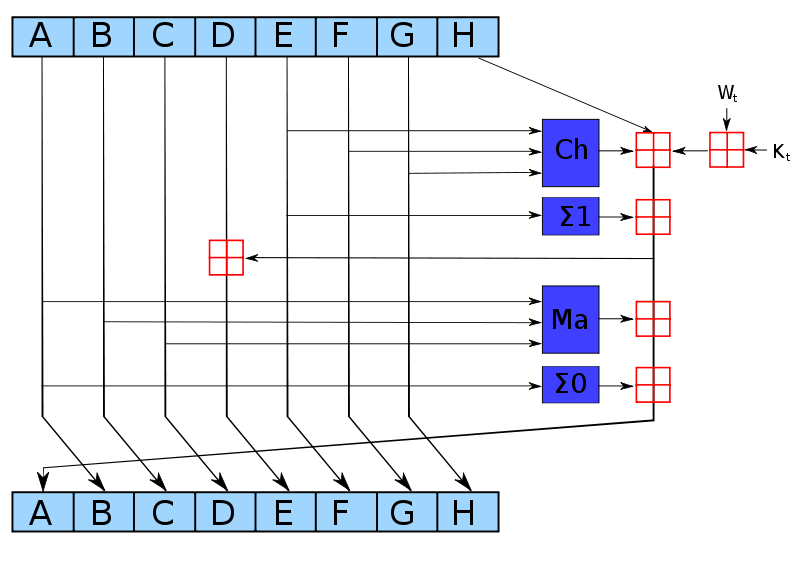
\includegraphics[height = 4 cm]{images/sha2.png}
		 	\caption{funzione di compressione $\orange{C}$}
	 	\end{figure}
	 \end{column}
	\end{columns}

\end{frame}